\begin{tikzpicture}[remember picture,overlay]
    \node[xshift=-0.8in,yshift=-0.8in,anchor=north east] at (current page.north east){%
    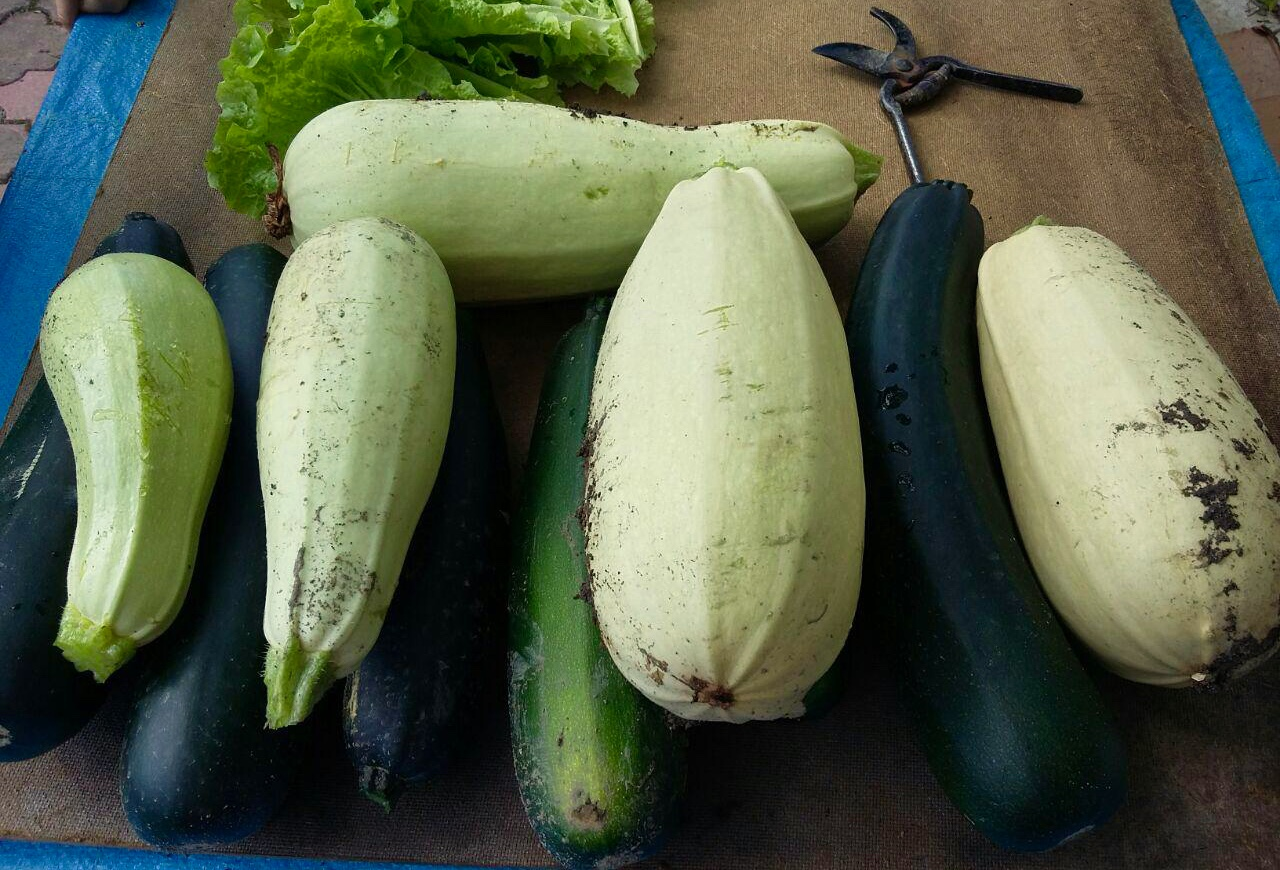
\includegraphics[width=6cm]{pic/leczo}};
\end{tikzpicture}


\begin{recipe}
    [% 
        preparationtime = {\unit[15]{min}},
        portion = {\portion{4}},
        bakingtime = {\unit[25]{min}}
    ]
    {Ratatouille \\ ~~or lecsó}


    \introduction{%
        When first courgettes appear in the allotment it is time for lecsó (and then for courgette ketchup but this is a story for another time).

        Our arbitrary decision was to call lecsó 'ratatouille with meat', so this is the distinction....If you want lecsó then, add fried sausage at the end of cooking ratatouille ;)

        Smoked paprika is \underline{essential}, all the taste is hidden here.

        If you can buy (or grow...) a marrow, exchange some of the courgettes for marrows. Remember that marrow usually requires peeling.
    }

    \ingredients[10]{%
        4 & Courgettes \\
        3 & Sweet longitudinal peppers \\
        1 & Red onion \\
        2 c. & Tomatoes \\
        2 tbs. & Smoked paprika \\
        2 tbs. & Paprika \\
        1 ts. & Hot paprika \\
        1 tbs. & Sugar
    }

    \preparation{%
        \step Dice onion, fry with all spices.
        Add peppers (big squares) and courgettes (quarter moons) and fry for 5 min.
        \step Add tomatoes, salt to taste, and cook for 5-8 min.
        \step Add fried sausage or chickpea.
        \step Serve with crusty bread.
    }

    \hint{%
        You can also add aubergines but as they need more time to cook,
        fry them for extra 4 min before adding other vegetables.
        There's also a creamy version available - add marrow, exchange peppers for carrots,
        reduce amount of smoked paprika, add cream and fresh herbs (eg.
        parsley or... lovage).
    }

\end{recipe}

% \begin{figure}[h]
%     \centering
%     \includegraphics[width=8cm]{}
% \end{figure}
